\documentclass[letterpaper,12pt,oneside]{article}\usepackage[]{graphicx}\usepackage[]{color}
%% maxwidth is the original width if it is less than linewidth
%% otherwise use linewidth (to make sure the graphics do not exceed the margin)
\makeatletter
\def\maxwidth{ %
  \ifdim\Gin@nat@width>\linewidth
    \linewidth
  \else
    \Gin@nat@width
  \fi
}
\makeatother

\definecolor{fgcolor}{rgb}{0.345, 0.345, 0.345}
\newcommand{\hlnum}[1]{\textcolor[rgb]{0.686,0.059,0.569}{#1}}%
\newcommand{\hlstr}[1]{\textcolor[rgb]{0.192,0.494,0.8}{#1}}%
\newcommand{\hlcom}[1]{\textcolor[rgb]{0.678,0.584,0.686}{\textit{#1}}}%
\newcommand{\hlopt}[1]{\textcolor[rgb]{0,0,0}{#1}}%
\newcommand{\hlstd}[1]{\textcolor[rgb]{0.345,0.345,0.345}{#1}}%
\newcommand{\hlkwa}[1]{\textcolor[rgb]{0.161,0.373,0.58}{\textbf{#1}}}%
\newcommand{\hlkwb}[1]{\textcolor[rgb]{0.69,0.353,0.396}{#1}}%
\newcommand{\hlkwc}[1]{\textcolor[rgb]{0.333,0.667,0.333}{#1}}%
\newcommand{\hlkwd}[1]{\textcolor[rgb]{0.737,0.353,0.396}{\textbf{#1}}}%

\usepackage{framed}
\makeatletter
\newenvironment{kframe}{%
 \def\at@end@of@kframe{}%
 \ifinner\ifhmode%
  \def\at@end@of@kframe{\end{minipage}}%
  \begin{minipage}{\columnwidth}%
 \fi\fi%
 \def\FrameCommand##1{\hskip\@totalleftmargin \hskip-\fboxsep
 \colorbox{shadecolor}{##1}\hskip-\fboxsep
     % There is no \\@totalrightmargin, so:
     \hskip-\linewidth \hskip-\@totalleftmargin \hskip\columnwidth}%
 \MakeFramed {\advance\hsize-\width
   \@totalleftmargin\z@ \linewidth\hsize
   \@setminipage}}%
 {\par\unskip\endMakeFramed%
 \at@end@of@kframe}
\makeatother

\definecolor{shadecolor}{rgb}{.97, .97, .97}
\definecolor{messagecolor}{rgb}{0, 0, 0}
\definecolor{warningcolor}{rgb}{1, 0, 1}
\definecolor{errorcolor}{rgb}{1, 0, 0}
\newenvironment{knitrout}{}{} % an empty environment to be redefined in TeX

\usepackage{alltt}
\usepackage[paperwidth=8.5in,paperheight=11in,top=1in,bottom=1in,left=1in,right=1in]{geometry}
\usepackage{setspace}
\usepackage[colorlinks=true,allcolors=Blue]{hyperref}
\usepackage[usenames,dvipsnames]{xcolor}
\usepackage{indentfirst}
\usepackage{titlesec}
\usepackage{multirow}
\usepackage{booktabs}
\usepackage{graphicx}
\usepackage{verbatim}
\usepackage{rotating}
\usepackage{tabularx}
\usepackage{outlines}
\usepackage{lineno}
\usepackage{array}
\usepackage{times}
\usepackage{cleveref}
\usepackage{acronym}
\usepackage[position=t]{subfig}
\usepackage{paralist}
\usepackage[noae]{Sweave}
\usepackage{natbib}
\usepackage{array}
\usepackage{pdflscape}
\usepackage{bm}
\usepackage{fixltx2e}
% \usepackage{showlabels}
\bibpunct{(}{)}{,}{a}{}{,}

% page margins and section title formatting
\linespread{1.5}
\setlength{\footskip}{0.5in}
\titleformat*{\section}{\Large\bf\em}
\titleformat*{\subsection}{\singlespace\large\bf}
\titleformat*{\subsubsection}{\singlespace\normalsize\bf\em}
\titlespacing{\section}{0in}{0in}{0in}
\titlespacing{\subsection}{0in}{0in}{0in}
\titlespacing{\subsubsection}{0in}{0in}{0in}

% cleveref options
\crefname{table}{Table}{Tables}
\crefname{figure}{Fig.}{Figs.}
\renewcommand{\figurename}{Fig.}

% aliased citations
\defcitealias{LehrterIR}{Lehrter et al. in review}

%acronyms
\acrodef{chla}[chl-\textit{a}]{chlorophyll \textit{a}}
\acrodef{cgem}[CGEM]{Coastal General Ecosystem Model}
\acrodef{do}[O$_2$]{dissolved oxygen}
\acrodef{gom}[GOM]{Gulf of Mexico}
\acrodef{lcs}[LCS]{Louisiana continental shelf}
\acrodef{marb}[MARB]{Mississippi-Atchafalaya River Basin}
\acrodef{oned}[1-D]{one-dimensional}
\acrodef{par}[PAR]{photosynthetically active radiation}

%for supplemental figures/tables
\newcommand{\beginsupplement}{%
        \setcounter{table}{0}
        \renewcommand{\thetable}{S\arabic{table}}%
        \setcounter{figure}{0}
        \renewcommand{\thefigure}{S\arabic{figure}}%
     }

%knitr options


% get the version based on commit date


% get online bib file


\IfFileExists{upquote.sty}{\usepackage{upquote}}{}
\begin{document}

\raggedbottom
\linenumbers
\raggedright
\urlstyle{same}
\setlength{\parindent}{0.5in}
\renewcommand\refname{References \vspace{12pt}}

\begin{singlespace}
\title{{\bf {\Large Title....}}}
\author{
  {\bf {\normalsize Marcus W. Beck$^1$, John C. Lehrter$^1$}}
  \\\\{\textit {\normalsize $^1$USEPA National Health and Environmental Effects Research Laboratory}}
  \\{\textit {\normalsize Gulf Ecology Division, 1 Sabine Island Drive, Gulf Breeze, FL 32561}}
	\\{\textit {\normalsize Phone: 850-934-2480, Fax: 850-934-2401}}
	\\{\textit {\normalsize Emails: \href{mailto:beck.marcus@epa.gov}{beck.marcus@epa.gov}, \href{mailto:lehrter.john@epa.gov}{lehrter.john@epa.gov}}}
  \vspace{1in} 
  \\ Version Date:   Wed Jun 29 16:36:46 2016 -0500
	}
\date{}
\maketitle
\end{singlespace}
\clearpage

\begin{abstract}
\noindent Bio-geo-chemical models are useful tools in environmental sciences that can guide management and policy-making. Consequently, significant time and resources are spent developing these models in system-specific contexts. The optimization of model parameters to maximize precision, including transferability of these models to different systems, are fundamental concerns in the development and application of these tools. This study describes quantitative limitations of coupled hydrodynamic-ecological modelling by contrasting numeric and ecological certainty with a systematic framework for characterizing parameter sensitivity and identifability.  We evaluate a simple bio-geo-chemical model that is the \ac{oned} unit of a larger spatio-temporal model of hypoxia on the \acl{lcs} of Gulf of Mexico as an example. Results from analysis of the \ac{oned} model are used to infer larger trends in dissolved oxygen dynamics over time, having implications for understanding factors that contribute to environmental conditions that are detrimental to aquatic resources.  In particular, we focus on issues of parameter identifiability using local sensitivity analyses to provide quantitative descriptions of numerical constraints on model precision.  We argue that quantitative and ecological certainty in model calibration are often at odds and the practitioner must explicitly choose model components to optimize given tradeoffs between the two. We further conclude that numerically optimal parameter sets for models of hypoxia are often small subsets of the complete parameter set because of redundancies in the unique effects of paramater perturbations on model output.  As a result, we demonstrate that use of a model for inference into ecological mechanisms of observed or predicted changes in hypoxic condition can be potentially misguided in the absence of quantitative descriptions of identifiability.  Although these concerns have been expressed in the literature, they are rarely explicitly addressed or included in model evaluations.  In addition to immediate implications for regional models, we provide a framework for describing the effects of parameter uncertainty and identifiability that can be applied to similar models to better inform environmental management.
\end{abstract}
\acresetall

\section{Introduction}

\begin{enumerate}
\item Simulation/biogeochemical/process-based models overview, contrast with statistical models
\item What models seek to provide - generality, precision, realism \cite{Levins66}, there is a tradeoff so models are 1) developed in partial independence and dependence on the world and theory, 2) function autonomously from both, or 3) represent both at the same time, from \cite{Morrison99}, cited in \cite{Ganju16}.  This is similar to the bias-variance tradeoff for statistical models, e.g., overparameterization of a model makes it very biased as it fits the data (the world) exactly, tradeoff between sensitity and error with changes in model complexity (more complexity is less error but increasing sensitivity) described in \cite{Snowling01}
\item How is model performance/uncertainty evaluated regarding what they should provide - structural, observational, parameter \cite{Beck87}?
\item Parameter uncertainy as low-hanging fruit - can do post-hoc and from inner to outer level of complexity, parameter uncertainty is the most common, e.g., marine ecological model \cite{Mateus15}, but stopped short, global sensitivity analysis of eutrophication model \cite{Estrada10}
\item Challenges related to uncertainty - similar to degrees of freedom, identifiability definition from \cite{Brun01} and need to evaluate identifiability \cite{Fasham06}, \cite{Omlin01} did a similar analysis with freshwater biogeochem model.
Identifiability describes the ability to estimate a parameter in relation to variation among the remaining parameters.  A parameter is identifiable if all parameters within the set can be uniquely estimated based on the observed data.  Parameters that are unidentifiable typically produce similar model outputs for a given relative perturbation, i.e., the effect of altering one parameter can be undone by altering one or more other parameters.  Model calibration will not converge for parameters sets that are unidentifiable. 
\end{enumerate}

This study describes a parameter sensitivity analysis to evaluate identifiability for a bio-geo-chemical model of hypoxia for the northern \ac{gom}.  We evaluate a simple \ac{oned} unit of a larger spatial-temporal model to explore relationships between multiple parameter sets and hypoxia dynamics on the \ac{lcs}.  The study also provides a general framework for sensitivity analysis and parameter identifiability that can be used on similar mechanistic models.  Specifically, an assumption is that models are generally over-parameterized and only a finite and smaller subset of the larger parameter set can be optimized for a given research question or dataset.  We provide explicit guidance for choosing such subsets of the parameter space given constraints on identifiability as directly related to sensitivity analyses.  The specific objectives are to \begin{inparaenum}[1\upshape)]
\item identify the parameters that have the greatest influence on \ac{do} using local sensitivity analysis,
\item quantify the identifiability of subsets of the total parameter space based on sensitivity,
\item provide a set of heuristics for choosing parameters based on sensitivity and parameter categories with the larger mechanistic model, including extension to other state variables, and 
\item discuss implications for hypoxia formation in coastal regions, including management strategies for nutrient reduction and use of mechanistic models to inform decision-making.
\end{inparaenum}
The `optimum' parameter space is defined as the chosen subset that represents the maximum number of identifiable parameters.  Here, `optimum' is both a qualitative description based on a research question or management goal and a quantitative objective based on numerical optimization criteria for fitting model output to a calibration dataset.  These results can be used to refine existing models or guide application of models to novel contexts, such as downscaling or application to new environments. 

\section{Methods}

\subsection{Model description}

Low concentrations of \acl{do} occur seasonally on the \ac{lcs} in the northern \ac{gom}.  These hypoxic events, defined as $<$2 mg L$^{-1}$ ($<$ 64 mmol m$^-3$ of O$_2$), occur in bottom waters and are caused by nutrient inputs from the \ac{marb} that drains a significant portion of the continental United States.  Nutrient-stimulated primary production in surface waters increases biological oxygen demand in bottom waters as sinking organic matter is decomposed.  The hypoxic area averages 15,540 km$^2$ annually (1993-2015) with minimum concentrations observed from late spring to early fall.  Seasonal variation is strongly related to carbon and nutrient export from the \ac{marb} \citep{Lohrenz08,Bianchi10}, whereas factors related to hydrologic variation and wind patterns can affect vertical salinity gradients that contribute to the formation of hypoxia \citep{Wiseman97}. 

Three-dimensional numerical simulation models have been developed to describe factors contributing to hypoxia and to predict the effects of management actions or climate scenarios on future patterns (\citealt{Fennel13,Pauer16}, \citetalias{LehrterIR}).  This study evaluates a recently developed hydrodynamic and ecological model that describes horizontal and vertical transport and mixing of state variables relevant for hypoxia.  The \ac{cgem} includes elements from the Navy Coastal Ocean Model \citep{Martin00} to describe hydrodynamics on the \ac{lcs} and a biogeochemical model with multiple plankton groups, water-column metabolism, and sediment diagenesis \citep{Eldridge10}.  The hydrodynamic component of \ac{cgem} provides a spatially-explicit description of hypoxia dynamics using an orthogonal grid with an approximate horizontal resolution of 1.9 km$^2$ and twenty equally-spaced vertical sigma layers on the shelf (depth $\leq$ 100 m, with additional hybrid layers at deeper depths).  The biogeochemical component includes equations for 36 state variables including six phytoplankton groups (with nitrogen and phosophorus quotas for each), two zooplankton groups, nitrate, ammonium, phosphate, dissolved inorganic carbon, oxygen, silica, and multiple variables for dissolved and particulate organic matter from different sources.  The model can be run for a set period of time at a given time step using atmospheric and hydrological boundary conditions described in \citet{Hodur97} and \citet{Lehrter13}.

The core unit of \ac{cgem} is a \ac{oned} model called FishTank that implements the biogeochemical equations in \citet{Eldridge10}.  This model acts as a standalone operational unit from the 3-D model that does not include any form of transport (i.e., advection, mixing, or surface flux) such that it can easily be applied to other hydrodynamic grids.  Accordingly, the sensitivity and identifiability analysis described below are informative for both the \ac{lcs} gridded model as well as potential applications to different systems.  The FishTank model provides estimates for the 36 state variables described above using a \ac{oned} parcel that is uniformly mixed.  A set of initial conditions is provided as input to the model that was based on observations of relevant variables obtained from research cruises in April, June, and September 2006 (Table 1, \citet{Murrell14}).  The FishTank model was executed from January 1\textsuperscript{st} to December \textsuperscript{st}, 2006 at a timestep of five minutes.  

Results from FishTank are based on time-dependent differential equations that describe energy flow between phytoplankton (up to six groups) and zooplankton (two groups) as affected by nutrient uptake rates, organic matter inputs and losses, inherent optical properties, sediment diagenesis, and temperature (\citealt{Penta08,Eldridge10}, see appendix in \citetalias{LehrterIR}).  A total of 108 equations are estimated at each time step to return a value for each of the 36 state variables described by the model.  In addition to the initial conditions, a set of parameter values for each of the equations is also supplied at model execution.  These parameters define relationships among fixed effects in the equations and represent ecological properties described by the model that influence hypoxia formation.  Values for each of the parameters were based on estimates from the literature, field or laboratory-based measurements, or expert-based knowledge in absence of the former.  The sensitivity of \ac{do} was estimated at each timestep from FishTank in relation to 249 parameters that are included in the 108 equations.  For simplicity in the discussion below, the parameters were grouped into one of six categories based on respective equations: optics, organic matter, phytoplankton, temperature, and zooplankton.  A full description of the equations and parameters is available as an appendix in \citepalias{LehrterIR}.  
\subsection{Local sensitivity analysis}

The analysis focused on sensitivity of \ac{do} in the \ac{oned} FishTank model to identify parameters that may affect spatial and temporal variation of hypoxia in the larger model.  A local sensitivity analysis was performed for each of the 249 parameters using a simple perturbation approach to evaluate the change in \ac{do} from the original parameter values.  The analyses relied exlusively on concepts used in the FME package developed for the R statistical programming language \citep{Soetaert10}. Each parameter was perturbed by 50\% of its original value and the model was executed to obtain an estimate of the effect on \ac{do}.  For each perturbation, a sensitivity value $S$ was estimated for each time step $i$ given a set value for parameter $j$ as:

\begin{equation} \label{sijeqn}
S_{ij} = \frac{\partial y_i}{\partial \Theta_j}\cdot\frac{w_{\Theta_j}}{w_{y_i}}
\end{equation}

\noindent where the estimate depended on the change in the predicted value for response variable $y$ divided by the change in the parameter $\Theta_j$ multiplied by the quotient of scaling factors $w$ for each.  The scaling factors, $w_{\Theta_j}$ for the parameter $\Theta_j$ and $w_{y_i}$ for response variable $y_i$, were set as the default value of the unperturbed parameter and the predicted value of $y_i$ after perturbation \citep{Soetaert10}.  The scaling ensures the estimates are unitless such that the relative magnitudes provide a comparison for model sensitivity to parameter changes that may vary in scale.  Estimates for $S_{ij}$ were summarized as $L1$ and $L2$ across the time series to obtain individual sensitivity values of \ac{do} in response to a change in parameter $j$:

\begin{equation} \label{l1}
L1 = \sum|S_{ij}|/n
\end{equation}
\begin{equation} \label{l2}
L2 = \sqrt{\sum\left(S_{ij}^2\right)|/n}
\end{equation}

In general, positive sensitivity estimates suggested a parameter had a positive effect on \ac{do} for a given increase in the parameter, whereas the converse was true for negative sensitivity estimates.  However, the effect of a parameter change may not be uniform over time such that $S_{ij}$ can change in magnitude and sign depending on the location.  Time series of \ac{do} estimates before and after perturbation were also evaluated to identify patterns not captured by the summary statistics. All parameters for each of the six equation categories (optics, organic matter, phytoplankton, temperature, and zooplankton) that had non-zero $L1$ or $L2$ were retained for identifiability analysis.  

\subsection{Identifiability and selecting parameter subsets}

Identifiability of parameter subsets was estimated from the minimum eigenvector of the cross-product of a selected sensitivity matrix \citep{Brun01,Omlin01}:

\begin{equation} \label{gameq}
\gamma = \frac{1} {\sqrt{ \min \left(\rm{EV}[\mathit{\hat{S}}^\top \mathit{\hat{S}}]\right)}}
\end{equation}

\noindent where $\gamma$ ranges from one to infinity for perfectly identifiable (orthogonal) or unidentifiable (perfectly collinear) results for a set of parameters in a chosen sensitivity matrix $S$.  The sensitivity functions were supplied as a matrix $\hat{S}$ with rows $i$ and columns $j$ (\cref{sijeqn}) that describes deviations of predicted \ac{do} from the default parameter values.  The matrix $\hat{S}$ was first normalized by dividing by the square root of the summed residuals\citep{Omlin01,Soetaert10}. 

The collinearity index $\gamma$ provides a measure of the linear dependence between sensitivity functions described above for subsets of parameters. Estimates of $\gamma$ greater than 10-15 suggest parameter sets are poorly identifiable \citep{Brun01,Omlin01}, meaning optimal values are inestimable given similar effects of the selected parameters on \ac{do}. Greater sensitivity of a state variable to parameters within a subset does not imply identifiability if the individual effects are similar.  An intuitive interpretation of $\gamma$ is provided by \citet{Brun01} such that a change in a state variable caused by a change in one parameter can be offset by the fraction $1 - 1/\gamma$ by the remaining parameters.  That is, $\gamma = 10$ suggests the relative change in \ac{do} for a selected parameter can be compensated for by 90\% with changes in the other parameters. 

Initial analyses suggested that considerably limited subsets of parameters were identifiable of the 249 included in the FishTank model.  Given this limitation, parameter selection must consider the competing objectives of increased precision with parameter inclusion and identifability as it relates to optimization.  An additional challenge is the excessively high number of combinations of parameter sets, which complicates selection given differences in parameter sensitivity and desired ecological categories of each parameter as they relate to the biogeochemical equations.  For example, \cref{fig:combnex} provides a simple graphic of the unique number of combinations that are possible for different subsets of `complete' parameter sets of different sizes (i.e., based on $n$ choose $k$ combinations equal to $n!/\left(k!\left(n-k\right)!\right)$).  The number of unique combinations increases with the total parameters in the set and is also maximized for moderate selections (e.g., selecting half the total).  For example, over 10$^14$ combinations are possible by selecting 25 parameters from a set of 50.  Accordingly, parameter selection is complicated by differing sensitivity, identifiability, and the difficulty of choosing from many combinations.

A set of heuristics was developed to balance the tradeoff in model complexity and identifiability given the challenges described above.  These rulesets were developed with the assumption that parameters will be selected given preference for those with high sensitivity and identifability based on $\gamma < 15$ was an acceptable threshold for subsets (e.g., 93\% accountability between parameters).  Selection heurestics also recognized that parameter categories (i.e., optics, organic matter, phytoplankton, temperature, zooplankton) may have unequal preferences given questions of interest.  In all selection scenarios, parameters were selected by decreasing sensitivity starting with the most sensitive until identifiability did not exceed $\gamma = 15$ where selections were \begin{inparaenum}[1\upshape)]
\item independent of parameter category,
\item blocked within parameter category,
\item or considering all categories equally
\end{inparaenum}.  The selection rules produced seven subsets of parameters that could further be used to optimize model calibration for \ac{do}.

Finally, the above analyses were repeated for additional state variables estimated by FishTank to provide further descriptions of ecological dynamics that are relevant for hypoxia.  In addition to \ac{do}, other state variables included \ac{chla}, \ac{par}, nitrate, ammonium, particulate organic matter, dissolved organic matter, and phosphorus.  Particulate and dissolved organic matter were estimated as the summation of the respective outputs for organic matter from phytoplankon (\textit{OM1\_A}, \textit{OM2\_A}), fecal pellets (\textit{OM1\_fp}, \textit{OM2\_fp}), river sources \textit{OM1\_rp}, \textit{OM2\_rp}), and boundary conditions (\textit{OM1\_bc}, \textit{OM2\_bc}, see \citetalias{LehrterIR}). 

\section{Results}

\subsection{Local sensitivity analysis}

\cref{tab:optsens,tab:tempsens,tab:phytosens,tab:zoopsens,tab:omsens}, how many parameters in each category, how many induced a response in \ac{do}, what parameters in each category had the greatest sensitivity (\cref{fig:sensplo}), what were sensitivity magnitudes between categories, did these vary by phyto or zoop groups?  

Plotting the raw values from the sensitivity analysis provides a visual assessment of changes (\cref{fig:sensplot}).

The identifiability functions evaluate the ability to identify all subsets from pairwise to all parameters in the subset.  As an example, the identifiability of pairwise combinations for each of the categories are shown below.

Pairwise identifiability of the top two most sensitive parameters in each category is shown, first as a table showing all unique combinations from two to all parameters and second as a figure showing pairwise combinations.

Reading each plot from left to right can be interpreted as including additional parameters, where each parameter is ranked by relative sensitivity.  The inset in each plot shows the identifiability of including parameters, up to a maximum where additional inclusion exceeds the identifability threshold of fifteen.  The scenarios for including parameters all begin with the parameters that have the greatest effect on the model output.  The inclusion of additional parameters depends on the scenario.  The first scenario selected parameters by decreasing sensitivity within each category (i.e., four separate models calibrated for optics, organics, phytoplankton, or zooplankton), the second scenario selected parameters by sensitivity regardless of category, and the third scenario selects parameters by sensitivity with equal representation between categories. 

\section{Discussion}

Questions specific to GOM - what initial conditions are important? How many phytoplankton groups do we need (e.g., related to structural uncertainty)?

How does the assimilation of additional parameters (e.g., other state variables) during calibration influence the conclusions?

How does uncertainty translate to what a model should provide (generality v precision)?  The first step - find out what can be optimized but then do not overfit....

What about structural uncertainty - does sensitivity of a model to variation in a parameter imply parameter uncertainty and/or structural uncertainty?

A final point about optimization with identifiable parameter sets - optimization to fit the data still does not ensure a correct model.  Failing in one way can be over-compensated by another feature, e.g., the parameter set that is optimized (see \cite{Flynn05}, p. 1207, third paragraph)

\cite{Omlin01} state that the sensitivity, identifiability, estimation process is iterative (p. 113), need to rinse and repeat for proper calibration. 

How to improve identifiability - get more/better observed data, include obs from other state variables in RSS minimization (eqn q in \cite{Omlin01})

Alternative methods for uncertainty analysis - bayesian, MCMC, nonlinear calibration-constrained optimization \citep{Gallagher07}

\clearpage
\begin{singlespace}
\bibliographystyle{apalike_mine}
\bibliography{refs}
\end{singlespace}
\clearpage

%%%%%%
% figures

% combination example
\begin{figure}[!ht]

{\centering 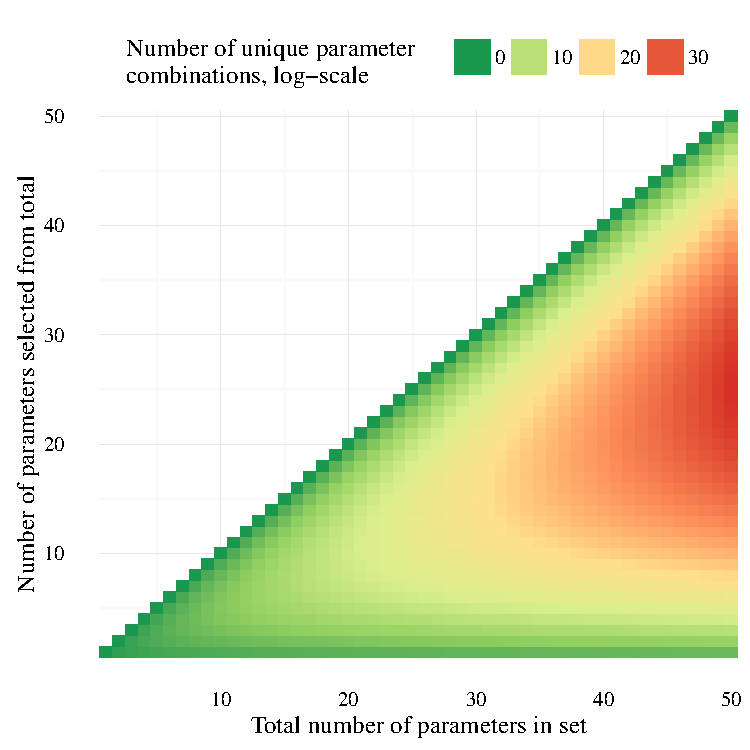
\includegraphics[width=0.6\textwidth]{figs/combnex-1} 

}

\caption[Examples of unique parameter combinations from different parameter sets and number of selected parameters]{Examples of unique parameter combinations from different parameter sets and number of selected parameters.  The number of combinations are shown for increasing numbers of selected parameters from the total in the set, where 50 parameter sets are shown each with one through 50 total parameters. Note that the number of unique combinations is shown as the natural-log.}\label{fig:combnex}
\end{figure}



% sensitivity example of top
\begin{figure}[!ht]

{\centering 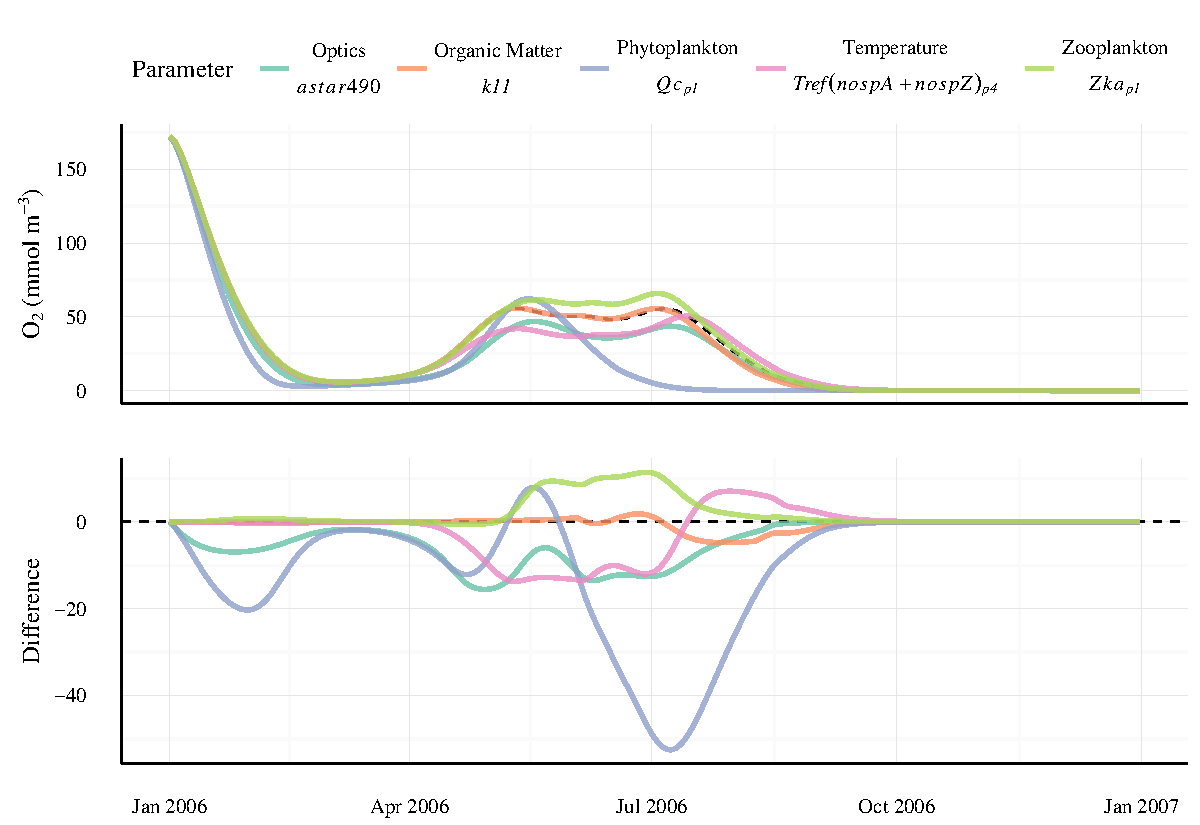
\includegraphics[width=\maxwidth]{figs/sensplo-1} 

}

\caption{Sensitivity of \ac{do} to parameter changes. The solid lines show the change in \ac{do} based on a 50\% change from the default parameter values (dashed line) for each parameter.  Individual parameters with the largest effect are shown for each category.  The top plot shows the model output and the middle plot shows the estimated \ac{do} as a difference from the default.  The bottom plot shows the distribution of error values (as $log\left(L1\right)$) for all parmaters in each category.}\label{fig:sensplo}
\end{figure}



% identifiability boxplots
\begin{figure}[!ht]

{\centering 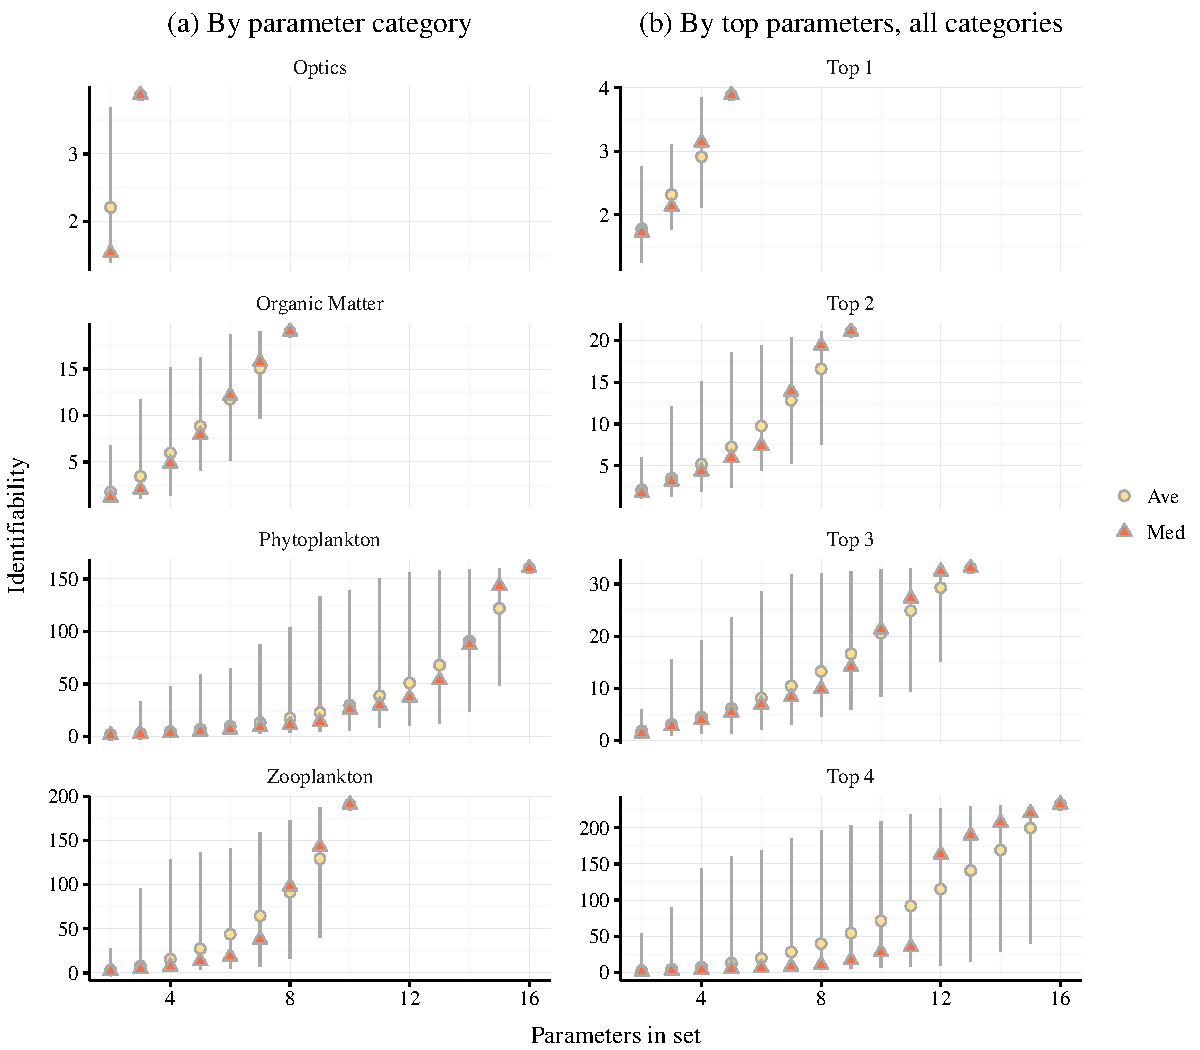
\includegraphics[width=\maxwidth]{figs/identbox-1} 

}

\caption[Identifiability (as ]{Identifiability (as $\gamma$, \cref{gameq}) of parameter subsets for \ac{do}.  Plots in (a) show identifiability by parameter caterogires (b) shows identifiability by seleting the top 1 through 5 parameters regardless of category.  Lines represent identifiability ranges for each the number of parameters in the set.  The phytoplankton category is limited to 25 total parameters.}\label{fig:identbox}
\end{figure}



\clearpage
%%%%%%
% tables

%latex.default(totab, file = "", rowlabel = "Description", caption = cap.val,     caption.loc = "top", rowname = Description, size = tabsize,     label = paste0("tab:", tablab))%
\begin{table}[!tbp]
{\normalsize
\caption{Sensitivities of \ac{do} to perturbation of optics parameters.  Sensitivities are based on a 50\% increase from the default parameter value, where $L1$ and $L2$ summarize differences in model output from the default (see \cref{l1,l2}).  Parameters that did not affect \ac{do} are not shown.\label{tab:optsens}} 
\begin{center}
\begin{tabular}{lllll}
\hline\hline
\multicolumn{1}{l}{Description}&\multicolumn{1}{c}{Parameter}&\multicolumn{1}{c}{Value}&\multicolumn{1}{c}{L1}&\multicolumn{1}{c}{L2}\tabularnewline
\hline
Chla specific absorption at 490 nm&\textit{astar490}&$0.04$&$1.64$&$8.64$\tabularnewline
OMA specific absorption at 490 nm&\textit{astarOMA}&$0.1$&$0.02$&$0.1$\tabularnewline
OMZ specific absorption at 490 nm&\textit{astarOMZ}&$0.1$&$0.01$&$0.01$\tabularnewline
AOP, light attenuation due to CDOM&\textit{Kcdom}&$0$&$3.18\times 10^{-6}$&$1.09\times 10^{-5}$\tabularnewline
\hline
\end{tabular}\end{center}}

\end{table}


%latex.default(totab, file = "", rowlabel = "Description", caption = cap.val,     caption.loc = "top", rowname = Description, size = tabsize,     label = paste0("tab:", tablab))%
\begin{table}[!tbp]
{\normalsize
\caption{Sensitivities of \ac{do} to perturbation of organic matter parameters.  Sensitivities are based on a 50\% increase from the default parameter value, where $L1$ and $L2$ summarize differences in model output from the default (see \cref{l1,l2}).  Parameters that did not affect \ac{do} are not shown.\label{tab:omsens}} 
\begin{center}
\begin{tabular}{lllll}
\hline\hline
\multicolumn{1}{l}{Description}&\multicolumn{1}{c}{Parameter}&\multicolumn{1}{c}{Value}&\multicolumn{1}{c}{L1}&\multicolumn{1}{c}{L2}\tabularnewline
\hline
rate constant for nitrification&\textit{k11}&$5$&$2.11$&$16.1$\tabularnewline
O2 concentration that inhibits denitrification&\textit{KstarO2}&$10$&$1.91$&$11.76$\tabularnewline
turnover rate for OM1A and OM1G&\textit{KG1}&$50$&$1.49$&$6.83$\tabularnewline
turnover rate for OM2A and OM2G&\textit{KG2}&$50$&$1.37$&$3.46$\tabularnewline
half-saturation concentration for NO3 used in denitrification&\textit{KNO3}&$10$&$1.24$&$7.98$\tabularnewline
half-saturation concentration for O2 utilization&\textit{KO2}&$10$&$0.56$&$1.92$\tabularnewline
decay rate of CDOM, 1/day&\textit{KGcdom}&$0.01$&$0.01$&$0.03$\tabularnewline
\hline
\end{tabular}\end{center}}

\end{table}


%latex.default(totab, file = "", rowlabel = "Description, Parameter",     caption = cap.val, caption.loc = "top", rgroup = unique(Description),     n.rgroup = as.numeric(table(Description)), rgroupTexCmd = NULL,     rowname = Parameter, size = tabsize, label = paste0("tab:",         tablab))%
\begin{table}[!tbp]
{\normalsize
\caption{Sensitivities of \ac{do} to perturbation of phytoplankton parameters.  Sensitivities are based on a 50\% increase from the default parameter value, where $L1$ and $L2$ summarize differences in model output from the default (see \cref{l1,l2}).  Parameters that did not affect \ac{do} are not shown.  Subscripts show the phytoplankton or zooplankton group that applies for the parameter. Parameters less than the 75\textsuperscript{th} percentile (0.59) for L1 were removed for brevity.\label{tab:phytosens}} 
\begin{center}
\begin{tabular}{llll}
\hline\hline
\multicolumn{1}{l}{Description, Parameter}&\multicolumn{1}{c}{Value}&\multicolumn{1}{c}{L1}&\multicolumn{1}{c}{L2}\tabularnewline
\hline
{coefficient for non-limiting nutrient}&&&\tabularnewline
~~\textit{aN\textsubscript{P1}}&$1$&$2.7$&$47.26$\tabularnewline
~~\textit{aN\textsubscript{P3}}&$1$&$0.66$&$3.16$\tabularnewline
\hline
{half-saturation constant for N}&&&\tabularnewline
~~\textit{Kn\textsubscript{P3}}&$5.93$&$1.15$&$9.22$\tabularnewline
~~\textit{Kn\textsubscript{P4}}&$1.13$&$0.62$&$2.5$\tabularnewline
\hline
{initial slope of the photosynthesis-irradiance relationship}&&&\tabularnewline
~~\textit{alpha\textsubscript{P4}}&$3.96\times 10^{-16}$&$1.61$&$7.46$\tabularnewline
~~\textit{alpha\textsubscript{P3}}&$6.19\times 10^{-17}$&$1.06$&$3.74$\tabularnewline
~~\textit{alpha\textsubscript{P5}}&$3.87\times 10^{-16}$&$0.81$&$5.54$\tabularnewline
\hline
{minimum N cell-quota}&&&\tabularnewline
~~\textit{QminN\textsubscript{P3}}&$1.27\times 10^{-8}$&$1.53$&$6.4$\tabularnewline
~~\textit{QminN\textsubscript{P4}}&$1.53\times 10^{-10}$&$0.91$&$2.76$\tabularnewline
~~\textit{QminN\textsubscript{P1}}&$6.08\times 10^{-9}$&$0.62$&$4.55$\tabularnewline
\hline
{mortality coefficient}&&&\tabularnewline
~~\textit{mA\textsubscript{P3}}&$0.03$&$2.98$&$14.34$\tabularnewline
~~\textit{mA\textsubscript{P4}}&$0.11$&$1.35$&$7.04$\tabularnewline
\hline
{N-uptake rate measured at umax}&&&\tabularnewline
~~\textit{vmaxN\textsubscript{P5}}&$1.4\times 10^{-9}$&$7.57$&$43.9$\tabularnewline
~~\textit{vmaxN\textsubscript{P4}}&$1.33\times 10^{-9}$&$2.88$&$16.56$\tabularnewline
~~\textit{vmaxN\textsubscript{P3}}&$8.11\times 10^{-8}$&$1.99$&$15.23$\tabularnewline
~~\textit{vmaxN\textsubscript{P1}}&$4.1\times 10^{-8}$&$0.84$&$2.92$\tabularnewline
\hline
{P-uptake rate measured at umax}&&&\tabularnewline
~~\textit{vmaxP\textsubscript{P3}}&$6.15\times 10^{-8}$&$2.23$&$9.89$\tabularnewline
~~\textit{vmaxP\textsubscript{P1}}&$2.68\times 10^{-8}$&$0.74$&$11.41$\tabularnewline
\hline
{phytoplankton basal respiration coefficient}&&&\tabularnewline
~~\textit{respb\textsubscript{P4}}&$0.02$&$3.1$&$26.48$\tabularnewline
~~\textit{respb\textsubscript{P3}}&$0.02$&$2.15$&$6.35$\tabularnewline
~~\textit{respb\textsubscript{P5}}&$0.02$&$0.81$&$8.61$\tabularnewline
\hline
{phytoplankton carbon/cell}&&&\tabularnewline
~~\textit{Qc\textsubscript{P1}}&$1.35\times 10^{-6}$&$328.35$&$2181.05$\tabularnewline
~~\textit{Qc\textsubscript{P3}}&$2.65\times 10^{-6}$&$232.8$&$1574.72$\tabularnewline
~~\textit{Qc\textsubscript{P2}}&$1.68\times 10^{-7}$&$4.08$&$61.25$\tabularnewline
~~\textit{Qc\textsubscript{P4}}&$4.54\times 10^{-8}$&$1.03$&$3.75$\tabularnewline
\hline
{phytoplankton growth respiration coefficient}&&&\tabularnewline
~~\textit{respg\textsubscript{P4}}&$0.1$&$0.98$&$7.37$\tabularnewline
\hline
\end{tabular}\end{center}}

\end{table}


%latex.default(totab, file = "", rowlabel = "Description, Parameter",     caption = cap.val, caption.loc = "top", rgroup = unique(Description),     n.rgroup = as.numeric(table(Description)), rgroupTexCmd = NULL,     rowname = Parameter, size = tabsize, label = paste0("tab:",         tablab))%
\begin{table}[!tbp]
{\normalsize
\caption{Sensitivities of \ac{do} to perturbation of temperature parameters.  Sensitivities are based on a 50\% increase from the default parameter value, where $L1$ and $L2$ summarize differences in model output from the default (see \cref{l1,l2}).  Parameters that did not affect \ac{do} are not shown.  Subscripts show the phytoplankton or zooplankton group that applies for the parameter.\label{tab:tempsens}} 
\begin{center}
\begin{tabular}{llll}
\hline\hline
\multicolumn{1}{l}{Description, Parameter}&\multicolumn{1}{c}{Value}&\multicolumn{1}{c}{L1}&\multicolumn{1}{c}{L2}\tabularnewline
\hline
{Optimum temperature for growth(C)}&&&\tabularnewline
~~\textit{Tref(nospA+nospZ)\textsubscript{P4}}&$17$&$2.9$&$22.95$\tabularnewline
~~\textit{Tref(nospA+nospZ)\textsubscript{Z2}}&$26$&$0.18$&$2.59$\tabularnewline
~~\textit{Tref(nospA+nospZ)\textsubscript{P5}}&$26$&$0.17$&$0.72$\tabularnewline
~~\textit{Tref(nospA+nospZ)\textsubscript{P2}}&$22$&$0.16$&$0.82$\tabularnewline
~~\textit{Tref(nospA+nospZ)\textsubscript{Z1}}&$22$&$0.16$&$0.33$\tabularnewline
~~\textit{Tref(nospA+nospZ)\textsubscript{P3}}&$17$&$0.14$&$0.78$\tabularnewline
~~\textit{Tref(nospA+nospZ)\textsubscript{P1}}&$22$&$0.12$&$0.29$\tabularnewline
\hline
\end{tabular}\end{center}}

\end{table}


%latex.default(totab, file = "", rowlabel = "Description, Parameter",     caption = cap.val, caption.loc = "top", rgroup = unique(Description),     n.rgroup = as.numeric(table(Description)), rgroupTexCmd = NULL,     rowname = Parameter, size = tabsize, label = paste0("tab:",         tablab))%
\begin{table}[!tbp]
{\normalsize
\caption{Sensitivities of \ac{do} to perturbation of zooplankton parameters.  Sensitivities are based on a 50\% increase from the default parameter value, where $L1$ and $L2$ summarize differences in model output from the default (see \cref{l1,l2}).  Parameters that did not affect \ac{do} are not shown.  Subscripts show the phytoplankton or zooplankton group that applies for the parameter.\label{tab:zoopsens}} 
\begin{center}
\begin{tabular}{llll}
\hline\hline
\multicolumn{1}{l}{Description, Parameter}&\multicolumn{1}{c}{Value}&\multicolumn{1}{c}{L1}&\multicolumn{1}{c}{L2}\tabularnewline
\hline
{assimilation efficiency as a fraction of ingestion}&&&\tabularnewline
~~\textit{Zeffic\textsubscript{P1}}&$0.4$&$0.23$&$0.55$\tabularnewline
~~\textit{Zeffic\textsubscript{P2}}&$0.4$&$0.21$&$0.75$\tabularnewline
\hline
{half saturation coefficient for grazing}&&&\tabularnewline
~~\textit{ZKa\textsubscript{P1}}&$1.12\times 10^{12}$&$0.82$&$6.29$\tabularnewline
~~\textit{ZKa\textsubscript{P2}}&$1.12\times 10^{12}$&$0.46$&$3.24$\tabularnewline
\hline
{maximum growth rate of zooplankton}&&&\tabularnewline
~~\textit{Zumax\textsubscript{P2}}&$2.98\times 10^{7}$&$0.48$&$1.84$\tabularnewline
~~\textit{Zumax\textsubscript{P1}}&$9.45\times 10^{8}$&$0.46$&$0.91$\tabularnewline
\hline
{proportion of grazed phytoplankton lost to sloppy feeding}&&&\tabularnewline
~~\textit{Zslop\textsubscript{P1}}&$0.25$&$0.12$&$0.33$\tabularnewline
\hline
{Zooplankton biomass-dependent respiration factor}&&&\tabularnewline
~~\textit{Zrespb\textsubscript{P1}}&$0.1$&$0.45$&$3.02$\tabularnewline
~~\textit{Zrespb\textsubscript{P2}}&$0.42$&$0.09$&$1.05$\tabularnewline
\hline
{zooplankton carbon/individual}&&&\tabularnewline
~~\textit{ZQc\textsubscript{P2}}&$7.08\times 10^{-7}$&$0.1$&$0.36$\tabularnewline
~~\textit{ZQc\textsubscript{P1}}&$3.13\times 10^{-4}$&$0.06$&$0.62$\tabularnewline
\hline
{Zooplankton growth-dependent respiration factor}&&&\tabularnewline
~~\textit{Zrespg\textsubscript{P1}}&$0.2$&$0.24$&$3.19$\tabularnewline
~~\textit{Zrespg\textsubscript{P2}}&$0.3$&$0.12$&$0.31$\tabularnewline
\hline
{Zooplankton mortality constant for quadratic mortality}&&&\tabularnewline
~~\textit{Zm\textsubscript{P2}}&$7.2\times 10^{-4}$&$0.33$&$2.85$\tabularnewline
~~\textit{Zm\textsubscript{P1}}&$7.2\times 10^{-4}$&$0.26$&$0.8$\tabularnewline
\hline
{zooplankton nitrogen/individual}&&&\tabularnewline
~~\textit{ZQn\textsubscript{P1}}&$6.95\times 10^{-5}$&$0.47$&$1.64$\tabularnewline
~~\textit{ZQn\textsubscript{P2}}&$1.57\times 10^{-7}$&$0.24$&$1.35$\tabularnewline
\hline
{zooplankton phosphorus/individual}&&&\tabularnewline
~~\textit{ZQp\textsubscript{P2}}&$8.53\times 10^{-9}$&$0.01$&$0.01$\tabularnewline
~~\textit{ZQp\textsubscript{P1}}&$3.77\times 10^{-6}$&$0$&$0$\tabularnewline
\hline
\end{tabular}\end{center}}

\end{table}




\end{document}
